\subsubsection{Варикап. Свойства, режимы работы, области применения}

Извиняюсь, не нашёл ничего в Степаненко и Гусеве. Поэтому вырезки из интернета:

Варикап – это специально сконструированный полупроводниковый диод, емкость которого меняется в широких пределах при изменении приложенного к р-n-перехода обратного напряжения, т.е. электрически управляемая емкость. В качестве управляемой ёмкости в данном случае выступает только барьерная ёмкость. Диффузионная ёмкость не подходит, т.к. она проявляется при прямом смещении.

ВФХ варикапа выражается следующей формулой: (как и для обычных барьерных емкостей)
$$
C_U = \frac{C_0}{(1 - U/\varphi_k)^\frac{1}{n}}
$$

где $C_0$ - ёмкость, соответствующая нулевому смещению, n = 3 для плавного, и 2 для резкого перехода.

Характер изменения емкости р-n-перехода в зависимости от приложенного напряжения $U_{rev}$ показан на рис:

\begin{center}
	\begin{figure}[h!]
		\center{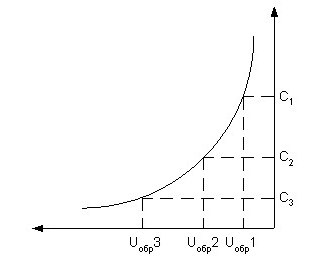
\includegraphics[scale=0.7]{VCUC.png}}
		\caption{}	
	\end{figure}
\end{center}

Важным свойством барьерной емкости является ее практическая безынерционность. Изменение барьерной емкости p-n-перехода при изменениии приложенного напряжения обусловлено смещением основных носителей заряда в прилегающих к барьерному слою областях. Скорость этого процесса очень велика, так как время перестройки объемного заряда в этом случае определяется временем максвелловской релаксации $\tau_r = \frac{\varepsilon\varepsilon_0}{qn\mu}$, где q - элементарный заряд, $\mu$ - его подвижность, n - концентрация. Для кремния, к примеру, время релаксации составляет $\approx 10^{-14}$с.

Эквивалентная схема варикапа:
\begin{center}
	\begin{figure}[h!]
		\center{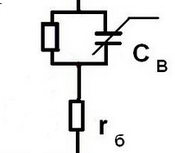
\includegraphics[scale=0.7]{vcs.png}}
		\caption{}	
	\end{figure}
\end{center}
(Кондёр шунтирует дифференциальное сопротивление)
На высоких частотах ёмкость шунтирует дифференциальное сопротивление и => можно представить эквивалентную схему просто как последовательное соединение сопротивления, отражающего объемное сопротивления тела базы и барьерного конденсатора.

Параметры варикапа:
\begin{itemize}
\item Добротность Q характеризует качество емкости диода, она определяется как отношение полного реактивного сопротивления к полному активному сопротивлению диода на заданной частоте. Добротность варикапа, определяемая для рекомендуемого режима на заданной частоте, называется номинальной и является важным параметром прибора.
\item Коэффициент перекрытия по емкости – $K_c$ в рабочем интервале обратных напряжений $K_c = \frac{C_{max}}{C_{min}}$
\item Предельная частота варикапа — значение частоты, на которой реактивная составляющая проводимости варикапа становится равной активной составляющей. Измерение предельной частоты производится при конкретных заданных обратном напряжении и температуре, которые в свою очередь зависят от типа варикапа.
\item Постоянный обратный ток — постоянный ток, протекающий через варикап при заданном обратном напряжении.
\item Максимально допустимое постоянное обратное напряжение.
\item Максимально допустимая рассеиваемая мощность.
\end{itemize}

Варикапы находят широкое применение для электронной подстройки резонансной частоты колебательных контуров. Изменяя напряжение на варикапе, подключенном к колебательному контуру, можно обеспечить дистанционное и безынерционнное управление резонансной частотой контура. 

Выглядит это примерно так:
\begin{center}
	\begin{figure}[h!]
		\center{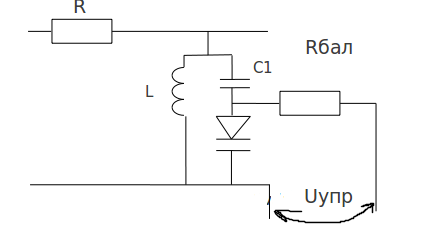
\includegraphics[scale=0.7]{VCLC.png}}
		\caption{}	
	\end{figure}
\end{center}

При подаче управляющего напряжения Uупр меняется емкость варикапа и как следствие резонансная частота.
